
\chapter{Potential Outcomes and Beyond}
\label{ch-pot-out}
This chapter
is based on Ref.\cite{book-mixtape},
a book by Stephen Cunningham entitled
\qt{Causal inference: the mixtape}.

The theory of potential
outcomes (PO) was for the most part
invented in a seminal
1974 paper by Donald B. Rubin. Rubin
has also
made important extensions
to PO theory since 1974. However, he
does not
use Pearl's causal DAGs to discuss PO theory.
Pearl has shown that PO theory
can be substantially clarified
and extended by using
the language of causal DAGs.
The d-separation theorem and do operator
that we discuss in  Chapters \ref{ch-dsep}
and \ref{ch-pot-out}
are especially
useful in this regard.
In this chapter, we stress the
connection
of PO theory to
Pearl's causal DAGs
and bnets.

\begin{table}[h!]
\centering
\begin{tabular}{|l|l|l|l|l|}
\hline
\rowcolor[HTML]{ECF4FF}
$\s$ & $ d^\s$ & $ y^\s$ & $ y^\s(0)$ & $ y^\s(1)$ \\ \hline
Edith & 0 & 5 & 5 & . \\ \hline
Frank & 0 & 7 & 7 & . \\ \hline
George & 0 & 8 & 8 & . \\ \hline
Hank & 0 & 10 & 10 & . \\ \hline
Andy & \cellcolor[HTML]{FFFFC7}1 & 10 & . & 10 \\ \hline
Ben & \cellcolor[HTML]{FFFFC7}1 & 5 & . & 5 \\ \hline
Chad & \cellcolor[HTML]{FFFFC7}1 & 16 & . & 16 \\ \hline
Daniel & \cellcolor[HTML]{FFFFC7}1 & 3 & . & 3 \\ \hline
\end{tabular}
\caption{PO dataset describing whether
individual $\s$
took a treatment drug ($d^\s=1$)
or didn't ($d^\s=0$).
The
treatment outcome
is measured by the real number $y^\s$.}
\label{tab-pot-out-missing}
\end{table}

Suppose a {\bf population
of individuals} $\s=0,1,2, \ldots, nsam-1$
is given ($d^\s=1$) or is
not given ($d^\s=0$)
a {\bf treatment dose} (i.e., {\bf treatment decision}) $d^\s$,
and that
the
 {\bf treatment outcome} (i.e., {\bf treatment response})
is measured by
a real number $y^\s$.
Table \ref{tab-pot-out-missing}
gives a possible {\bf PO dataset}
for this scenario.
As you
can see from
that table,
each individual
either takes a drug or
doesn't,
but not both.
PO theory
can be viewed as a
 {\bf  missing
data (MD) problem}. MD problems are
discussed in
 Chapter \ref{ch-missing-d}.
However, the PO MD problem
is much more specialized
than the generic MD problems
discussed in Chapter \ref{ch-missing-d}.
In the PO MD
problem, we can
fill
in the blank cells
by matching
each individual
that took
the drug with
another {\it similar}
individual that didn't.
We will have much
more to say about
this matching
strategy later in this chapter.

One can define
similar
individuals as
individuals that have the same
value
for $nx$ features $x^\s=(x^\s_i)_{i=0, 1, \ldots, nx-1}$.
One
can add to Table \ref{tab-pot-out-missing}
 $nx$ extra columns
giving the value of
the feature vector $x^\s$
for each individual.
Members
of a population with
the same $x^\s$
are referred to as
a
{\bf subpopulation or stratum (i.e., layer)}.

In a {\bf randomized controlled trial (RCT)}
\footnote{The term {\bf A/B test}
is often used to mean an RCT
where A and B are the treated and control groups. However,
sometimes the term is used to refer to
an experiment  that conditions on confounders,
which violates the definition of an RCT,
and is the same as a PO test.},
the effect
of the variable $x^\s$ on
the value
of $d^\s$
is eliminated by
randomizing
the population
and therefore
making the effect of $x^\s$
on $d^\s$
average out  to zero.
However,
there are many situations
in which carrying out an RCT is not
possible
or desirable. PO theory is
a way of predicting the
result
of an RCT in situations where
doing a real RCT is not possible
or desirable.

In this chapter, $x^\s$
will be called the confounders.
Implicit throughout this chapter
is the assumption that there are {\bf
no unmeasured confounders}.
Because if
there are some unmeasured confounders,
those can
send secret messages
that influence the value
that $d^\s$ takes.
This would ruin
the
predictions
of someone trying
to predict the results of an RCT
without
being privy to those secret
messages.
When there are {\bf some
unmeasured confounders},
it might still be
possible
to
predict the effect of an RCT.
This might be possible
using instrumental variables. See Chapter
\ref{ch-instrumental}
for a discussion
of {\bf instrumental
variables}.


\section{$G$ and $G_{den}$
bnets,
the starting point bnets}


\begin{figure}[h!]
$$
\begin{array}{ccc}
\xymatrix{
&\rvx^\s\ar[dl]\ar[dr]
\\
\rvd^\s\ar[rr]&&\rvy^\s
}
&&
\xymatrix{
u_\rvd\ar[dd]&u_\rvx\ar[d]&u_\rvy\ar[dd]
\\
&\rvx\ar[dl]\ar[dr]
\\
\rvd\ar[rr]&&\rvy
}
\\
\\
G&&G_{den}
\end{array}
$$
\caption{Bnets
$G$ and $G_{den}$
are
our starting
point in discussing PO theory.
 $G$ is for
a single individual $\s$ of the
population.
Bnet $G_{den}$ is the
DEN counterpart
to $G$.
DEN (Deterministic with
External Noise) bnets are discussed in Chapter
\ref{ch-LDEN}.}
\label{fig-po-G-start}
\end{figure}

In this chapter, we will
abbreviate
$\rvX[\s]=\rvX^\s$
for
$X\in \{d, x, y\}$, where
 $\s\in\{0,1,2, \ldots, nsam-1\}$.


For each individual (a.k.a. unit, sample)
$\s=0, 1, 2, \ldots nsam-1$, let:

$\rvd^\s\in\bool$ be the
 treatment dose or drug dose.
It equals 1 if
treated
and 0 if untreated.

$\rvy^\s\in \RR$ be the
 treatment potential outcome

$\rvx^\s$ be the column vector of treatment
confounders
(a.k.a. covariates because they
are often used as covariates (i.e.,
independent
variables) in linear regression.)

Consider bnets $G$ and $G_{den}$
in
 Fig.\ref{fig-po-G-start}.
$G$ reflects the language
used in Ref.\cite{book-mixtape}
to discuss PO theory. And
$G_{den}$ reflects
the language that Judea Pearl
prefers to use to discuss PO theory.
Both languages are equivalent. To go from
one language to the other, one need only
perform the following
swaps, where $\rvu$
is the external noise of the DEN bnet.

$\rvX^\s\leftrightarrow \rvX(\rvu)$
for $X\in \{d, x, y\}$.

$P(\s)=\frac{1}{nsam}\leftrightarrow P(u)$

$\sum_\s P(\s) (\cdot)
\leftrightarrow \sum_uP(u) (\cdot)$




The TPMs, printed in blue,
for the bnet
$G$
in Fig.\ref{fig-po-G-start},
are as follows:


\beq\color{blue}
P(x^\s)=
P_{\rvx}(x^\s)
\eeq

\beq\color{blue}
P(d^\s|x^\s)=
P_{\rvd|\rvx}(d^\s|x^\s)
\eeq


\beq\color{blue}
P(y^\s| d^\s, x^\s)=
P_{\rvy|\rvd, \rvx}(y^\s|d^\s, x^\s)
\eeq




Now let:

$\rvd\in\bool$
be the treatment dose.
It equals
1 if treated and 0 if untreated

$\rvy\in \RR$ be the
 treatment potential outcome

$\rvx$ be the column vector of
treatment
confounders (a.k.a. covariates)


$\rvu=(\rvu_\rvd,
\rvu_\rvx, \rvu_\rvy)$ be the
external noise

The TPMs, printed in blue,
for the bnet
$G_{den}$
in Fig.\ref{fig-po-G-start},
are as follows:


\beq \color{blue}
P(x|u_\rvx)= \indi(\;\;x=u_\rvx\;\;)
\eeq

\beq\color{blue}
P(d|x, u_\rvd)=
\indi( \;\; d= f_\rvd(x, u_\rvd)
\;\;)
\eeq

\beq\color{blue}
P(y|d,x, u_\rvy)=
\indi( \;\; y= f_\rvy(d,x, u_\rvy)
\;\;)
\label{eq-y-is-fy}
\eeq

If we linearize
 $f_\rvy$ in Eq.(\ref{eq-y-is-fy}),
we get

\beqa
\rvy =
\delta \rvd + \beta \rvx + \rvu_\rvy
\;,
\label{eq-y-is-lin}
\eeqa
where $\delta, \beta\in \RR$.
Assuming
that $\rvx, \rvy\in \RR$
and $\rvd\in \bool$,
Eq.(\ref{eq-y-is-lin}) can be plotted.
The resulting plot
is given in Fig.\ref{fig-po-two-parallel-lines}.
This plot
is a very special
case of the PO problem,
but it gives a crude idea
of the \qt{effects} $\delta
= y(1)-y(0)$ that PO theory
gives estimates for.
Any
individual participating in the experiment
experiences either $y(1)$
or $y(0)$,
but not both.



\begin{figure}[h!]
\centering
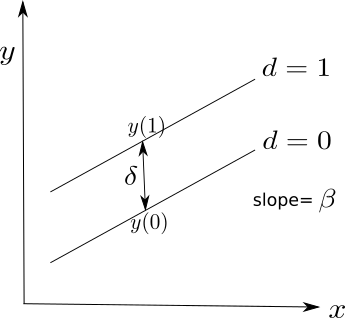
\includegraphics[width=2in]
{pot-out/two-parallel-lines.png}
\caption{Plot  of
Eq.(\ref{eq-y-is-lin})}
\label{fig-po-two-parallel-lines}
\end{figure}






\section{$G$ bnet
with nodes $y^\sigma(0),
y^\sigma(1)$ added to it.}


\begin{figure}[h!]
$$
\begin{array}{ccc}
\xymatrix{
&\rvx^\s\ar[ddl]\ar[ddr]
\\
\\
\rvd^\s\ar[rr]&&\rvy^\s
}
&
\xymatrix{
&&\rvx^\s\ar[ddll]\ar[d]
\\
&&[\rvy^\s(0),\rvy^\s(1)]\ar[d]
\\
\rvd^\s\ar[urr]^?\ar[rr]
&
&\rvy^\s
}
\\
G&G_{+}
\end{array}
$$
\caption{
Bnet $G_+$ is bnet $G$
with two new variables $\rvy^\s(0)$
and $\rvy^\s(1)$
added to it as a tuple node $[\rvy^\s(0), \rvy^\s(1)]$.
}
\label{fig-po-G-im-y0-y1}
\end{figure}

\begin{figure}[h!]
$$
\begin{array}{ccc}
\xymatrix@C=.1pc{
\rvx^\s\ar[d]
\\
[\rvy^\s(0),\rvy^\s(1)]\ar[d]
\\
\rvy^\s
}
&
\xymatrix@C=.1pc{
&\rvx^\s\ar[dl]\ar[dr]
\\
\rvy^\s(0)\ar[dr]
&& \rvy^\s(1)\ar[dl]
\\
&\rvy^\s
}
&
\xymatrix{
\rvx^\s\ar[d]
\\
\rvy^\s(\rvc^\s)\ar[d]
&\rvc^\s\ar[l]
\\
\rvy^\s
}
\\
(a)&(b)&(c)
\end{array}
$$
\caption{$(a), (b), (c)$ are 3 equivalent ways of
adding the variables $\rvy^\s(0)$,
$\rvy^\s(1)$ to graph $G$
to obtain $G_+$
in Fig.\ref{fig-po-G-im-y0-y1}.
Note that $c^\s\in \bool$.}
\label{fig-3-ways-y0-y1}
\end{figure}


Consider Fig.\ref{fig-po-G-im-y0-y1}.
Bnet $G_+$
 was obtained by adding a tuple node
$[\rvy^\s(0), \rvy^\s(1)]$
to bnet $G$.
Fig.\ref{fig-3-ways-y0-y1}
shows 3 equivalent ways of
adding the variables $\rvy^\s(0)$,
$\rvy^\s(1)$ to graph $G$
to obtain $G_+$.
The
TPMs, printed in blue,
 for bnet $G_+$,
are as follows. Note
that we define them in terms
of the TPMs
for bnet $G$.

\beq\color{blue}
P(x^\s)=
P_{\rvx}(x^\s)
\eeq

\beq\color{blue}
P(d^\s|x^\s)=
P_{\rvd|\rvx}(d^\s|x^\s)
\eeq

For $c\in \bool$,

\beq\color{blue}
P(y^\s(c)|d^\s, x^\s) =
\left\{
\begin{array}{ll}
P_{\rvy(c)|\rvd, \rvx}(y^\s(c)|d^\s, x^\s)
& \text{ if INCLUDE arrow  with question mark}
\\
P_{\rvy(c)| \rvx}(y^\s(c)|x^\s)
& \text{ if EXCLUDE arrow with question mark}
\end{array}
\right.
\eeq

\begin{subequations}
\label{eq-y-equal-ytd}
\beqa\color{blue}
P(y^\s|y^\s(0), y^\s(1), d^\s)=
&=&\color{blue}
\indi(y^\s= d^\s y^\s(1) + (1-d^\s)y^\s(0))
\\
&=&\color{blue}
\indi(y^\s= y^\s(d^\s))
\eeqa
\end{subequations}

Eq.(\ref{eq-y-equal-ytd})
is often referred to as the {\bf SUTVA or Consistency assumption}.

If we sum over the
nodes $\rvy(0)$ and $\rvy(1)$
of this bnet, we should
get the bnet $G$.
This is easy to check. Indeed,\footnote{To
convince yourself that Eq.(\ref{eq-y-is-y-td})
 is correct, note this.
If $d^\s=0$, you can sum over
$y^\s(1)$ firstly, thus
setting $\sum_{y^\s(1)}P(y^\s(1)|d^\s, x^\s)=1$.
Secondly, you can sum over $y^\s(0)$.}

\begin{align}
P(y^\s|d^\s, x^\s)
&=
\sum_{y^\s(0)}
\sum_{y^\s(1)}
\indi(y^\s= y^\s(d^\s))
P(y^\s(0)|d^\s, x^\s)
P(y^\s(1)|d^\s, x^\s)
\\
&=
\left\{
\begin{array}{ll}
P_{\rvy(0)|\rvd, \rvx}(
y^\s|d^\s, x^\s)&\text{ if }
d^\s=0
\\
P_{\rvy(1)|\rvd, \rvx}(
y^\s|d^\s, x^\s)&\text{ if }
d^\s=1
\end{array}
\right.
\;.
\label{eq-y-is-y-td}
\end{align}

Henceforth,
we will refer
to the case where
the question mark
arrow is included as
the general case,
and to the case when it's excluded
as the {\bf weak-d limit}.
Henceforth, we
will first present
results for the
general case,
and then
describe how  those
results
change for the
weak-d limit.
Rubinologists
always assume the
weak-d limit, but
we find that
with little effort,
we can derive
many results for
general case, and
then compare those
results
to their weak-d limit.
I find such
comparisons instructive.

Note that in the general case,
$P(\rvy(c)=y|\rvd=d, x)$
for $c, d\in \bool$
are four
different probability
distributions,
and that
$P(\rvy=y|d=d,x)$
is defined in terms
of two of them, the
so-called {\bf factual
distributions} with $c=d$.
By measuring $\rvy$,
we cannot access the other
2 probability distributions,
the so-called {\bf counter-factual
distributions}
with $c\neq d$.

In the weak-d limit,
$P(\rvy(c)=y|\rvd=d, x
)=P(\rvy(c)=y|x)$ are
two probability
distributions,
and they both
can be accessed
by measuring $\rvy$.





\section{Expected Values of
 treatment outcome $y^\sigma$}

It is convenient
to define
the following
expected values of
$\rvy^\s$
in terms of the TPMs of
bnet $G_{+}$:

\beq
\caly_{c| d,x}
=
E_{\s| d,x}[\rvy^\s(c)]
\rarrow
E_{ \rvy(c)| d,x} [\rvy(c)]
=\sum_{y} y
P(\rvy(c)=y|\rvd= d,x)
\label{eq-need-positivity}
\eeq

\beq
\caly_{c| d}
=
E_{\s| d}[\rvy^\s(c)]
\rarrow
E_{ \rvy(c)| d} [\rvy(c)]
=\sum_x\caly_{c|d,x}P(x|d)
\eeq

\beq
\caly_{c| x}
=
E_{\s| x}[\rvy^\s(c)]
\rarrow
E_{ \rvy(c)| x} [\rvy(c)]
=\sum_d\caly_{c|d,x}P(d|x)
\eeq


\beq
\caly_c=
E_{\s}[\rvy^\s(c)]
\rarrow
E_{\rvy(c)} [\rvy(c)]=
\sum_{x,d}\caly_{c|d,x} P(x,d)
\eeq

Note that in the weak-d limit,


\beq
\caly_c=\sum_x \caly_{c|d,x}P(x)
\;.
\eeq
Note also that in the weak-d limit,
$\caly_{c|d, x}$ is independent
of $d$,
but $\caly_{c|d}$
can depend on $d$
if $P(x|d)$ depends on $d$.


For $\caly_{c|d}$, the expected values $\caly_{0|0}, \caly_{1|1}$
are said to be {\bf factual}
(indicating compliant patients)
whereas
$\caly_{0|1}, \caly_{1|0}$
are said to be {\bf counterfactual}
(indicating non-compliant patients).

Also let

\beq
\caly_{| d,x}
=
E_{\s| d,x}[\rvy^\s]
\rarrow
E_{\rvy| d,x} [\rvy]
=\sum_{y} y
P(\rvy=y|\rvd= d,x)
\eeq


\beq
\caly_{| d}
=
E_{\s| d}[\rvy^\s]
\rarrow
E_{\rvy| d} [\rvy]
=\sum_x\caly_{|d,x}P(x|d)
\eeq

\beq
\caly_{| x}
=
E_{\s| x}[\rvy^\s]
\rarrow
E_{\rvy| x} [\rvy]
=\sum_d\caly_{|d,x}P(d|x)
\eeq

\beq
\caly
=
E_{\s}[\rvy^\s]
\rarrow
E_{\rvy} [\rvy]
=\sum_d\caly_{|d,x}P(d,x)
\eeq


In the weak-d limit,
$\caly_{|d,x}$ is independent
of $d$, but
$\caly_{|d}$ can still depend on  $d$
if $P(x|d)$ depends on $d$.




\section{Translation Dictionary}

{\renewcommand{\arraystretch}{1.5}
\begin{table}[h!]
\centering
\begin{tabular}{|l|l|}
\hline
\rowcolor[HTML]{ECF4FF}
In standard PO notation&
In our notation \\
\hline
$i$, individual (i.e., unit, sample) index& $\s$ \\
\hline
$D_i=d_i$, treatment dose & $\rvd^\s=d^\s$\\
\hline
$Y_i=y_i$, treatment outcome& $\rvy^\s=y^\s$ \\
\hline
$X_i=x_i$, treatment confounders& $\rvx^\s=x^\s$ \\
\hline
$E[Y_i(c)]$ &
$E_{\s}[\rvy^\s(c)]=\caly_{c}$ \\
\hline
$E[Y_i(c)|D_i= d]$ &
$E_{\s| d}[\rvy^\s(c)]=\caly_{c| d}$\\
\hline
$E[Y_i(c)|D_i= d, X_i=x]$ &
$E_{\s| d,x}[\rvy^\s(c)]=\caly_{c| d,x}$\\
\hline
$E[Y_i]$ &
$E_{\s}[\rvy^\s]=\caly$ \\
\hline
$E[Y_i|D_i= d]$ &
$E_{\s| d}[\rvy^\s]=\caly_{| d}$\\
\hline
$E[Y_i|D_i= d, X_i=x]$ &
$E_{\s| d,x}[\rvy^\s]=\caly_{| d,x}$\\
\hline
\end{tabular}
\caption{Dictionary for
translating
from standard PO notation
of Ref.\cite{book-mixtape}
to our notation. $c, d\in \bool$.
}
\label{tab-pot-out-dict}
\end{table}
}

Table \ref{tab-pot-out-dict}
gives a dictionary for
translating
from the standard PO notation
of Ref.\cite{book-mixtape}
to our notation.


\section{${\cal Y}_{|d,x}
={\cal Y}_{d|d,x}$ (SUTVA)}


\begin{claim}\footnote{In the
standard PO notation,
this is the frequently used identity
$$E[Y|D=d, x]= E[Y(d)|D=d, x]$$.
}
\label{cl-caly-bardx}

\beq
\caly_{| d, x}=\caly_{ d| d,x}
\label{eq-y-to-yd-x}
\eeq

\beq
\caly_{| d}=\caly_{ d| d}
\label{eq-y-to-yd}
\eeq

\end{claim}
\proof

\beqa
\caly_{| d,x}
&=&
\sum_y y P(\underbrace{\rvy}_
{=\rvy( d)
\text{ by Eq.(\ref{eq-y-equal-ytd})}}
=y| d, x)
\\
&=&
\caly_{ d| d, x}
\;.
\eeqa
Applying $\sum_x P(x|d)$ to
both sides
of Eq.(\ref{eq-y-to-yd-x})
gives
Eq.(\ref{eq-y-to-yd}).
\qed



\section{Conditional Independence Assumption (CIA)}

The {\bf Conditional Independence Assumption}
 (CIA)
is said to hold
 if\footnote{See Section \ref{sec-perp-p} for definition
 of $\perp_P$
 and $\perp_P^{sep}$}
\beq
(\rvy^\s(0), \rvy^\s(1))\perp_P^{sep}\rvd^\s | \rvx^\s
\;.
\label{eq-CIA2}
\eeq
This is satisfied by $G_+$
in the weak-d limit. This
follows immediately by
applying the d-separation theorem
(see Chapter \ref{ch-dsep})
to $G_+$. Indeed,
conditioning on $\rvx^\s$
blocks signals from entering
$[\rvy^\s(0), \rvy^\s(1)]$
through the path that passes through $\rvx^\s$.
Furthermore, $\rvy^\s$ acts as a collider, blocking the
path to $[\rvy^\s(0), \rvy^\s(1)]$ going
through $\rvy^\s$.

I think CIA only makes sense
if the individuals
are treatment blind (i.e.,
have no knowledge
of whether they are
in the treated or control
groups.) Otherwise,
that extra knowledge
becomes a
confounder not being
included in $x$.

A {\bf Randomized Controlled Trial (RCT)}
is defined to satisfy
Eq.(\ref{eq-CIA2}) without the
 $\rvx^\s$ conditioning; i.e., it
satisfies

\beq
(\rvy^\s(0), \rvy^\s(1))\perp_P^{sep}\rvd^\s
\;.
\label{eq-CIA-minus-x}
\eeq
This means that in an RCT,
the arrow from
$\rvx^\s$ to  $\rvd^\s$ in $G_+$
is omitted.

Note that
if we assume both CIA (i.e.,
weak-d limit)
and SUTVA, we get

\begin{subequations}
\beqa
\caly_{|d,x}
&=&
E_{\s|d,x}[\rvy^\s]
\\
&=&
E_{\s}[\rvy^\s|\rvd^\s=d, \rvx^\s=x]
\\
&=&
E_{\s}[\rvy^\s(d)|\rvd^\s=d, \rvx^\s=x]
\text{ (by SUTVA)}
\\
&=&
E_{\s}[\rvy^\s(d)|\rvx^\s=x]
\text{ (by CIA)}
\\
&=&
E_{\s|x}[\rvy^\s(d)]
\\
&=&
\caly_{d|x}
\;.
\label{eq-d-td-diff}
\eeqa
\end{subequations}
In an RCT, Eq.(\ref{eq-d-td-diff})
is valid without the $x$ conditioning.


\section{Treatment Effects}

\begin{figure}[h!]
\centering
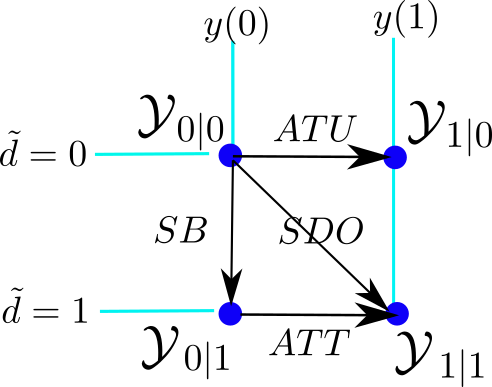
\includegraphics[height=1.8in]
{pot-out/y-diffs-square.png}
\caption{Different treatment effects.
A treatment effect is a difference of
two $\caly_{c| d }$.}
\label{fig-y-diffs-square}
\end{figure}

\begin{figure}[h!]
\centering
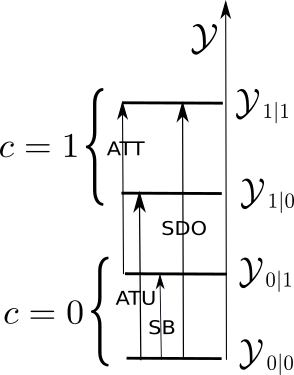
\includegraphics[width=1.6in]
{pot-out/po-y-levels.png}
\caption{Alternative
representation of the same
information that is contained in
Fig.\ref{fig-y-diffs-square}.}
\label{fig-po-y-levels}
\end{figure}

A {\bf treatment effect} is a
difference of two  $\caly_{c| d }$.
It is convenient to
define the following
treatment effects.
See Figs.\ref{fig-y-diffs-square}
and \ref{fig-po-y-levels}.




\begin{itemize}


\item average treatment effect
 (ATE).
\beq
{\color{red}ATE}=
\caly_{1}-
\caly_{0}= \delta
\eeq

\item average treatment effect
of the treated (ATT)
\beq
{\color{red}ATT}=
\caly_{1|1}-\caly_{0|1}
\eeq


\item average
treatment effect of the untreated (ATU)
\beq
{\color{red}ATU}=
\caly_{1|0}-\caly_{0|0}
\eeq

\item selection bias (SB)
\beq
{\color{red}SB}=\caly_{0|1}-\caly_{0|0}
\eeq


\item simple difference in outcomes (SDO)
\beq
{\color{red} SDO}= \caly_{1|1}-\caly_{0|0}
\eeq


\end{itemize}



Let

\beq
\pi_d = P(\rvd=d)
\eeq
for $d\in \bool$.

Note that there
exist some linear
constraints between
these treatment effects.



\beqa
\underbrace{\caly_1-\caly_0}_
{ATE}
&=&
\underbrace{
\caly_{1|1}\pi_1 +\caly_{1|0}\pi_0}_
{\caly_1}
-
\underbrace{(
\caly_{0|1}\pi_1 + \caly_{0|0}\pi_0)}_
{\caly_0}
\\
&=&
 \underbrace{(\caly_{1|1}-\caly_{0|1})}_{ATT}\pi_1+
 \underbrace{(\caly_{1|0}-\caly_{0|0})}_{ATU}\pi_0
\label{eq-ate-att-atu}
\eeqa

\beq
\underbrace{\caly_{1|1}-\caly_{0|0}}_{SDO}
=
\underbrace{(\caly_{1|1}-\caly_{0|1})}_{ATT}
+
\underbrace{\caly_{0|1}-\caly_{0|0}}_{SB}
\eeq

\beqa
\underbrace{\caly_{1|1}-\caly_{0|0}}_{SDO}
&=&
\underbrace{(\caly_{1|1}-\caly_{0|1})\pi_1 +
(\caly_{1|0}-\caly_{0|0})\pi_0 }_{ATE} \nonumber
\\
&&+
\underbrace{\caly_{0|1}-\caly_{0|0}}_{SB}\nonumber
\\
&&+
\underbrace{(\caly_{1|1}-\caly_{0|1})}_{ATT}\pi_0\nonumber
\\
&&-
\underbrace{(\caly_{1|0}-\caly_{0|0})}_{ATU}\pi_0
\label{eq-sdo-ate-else}
\eeqa

By virtue of  Eq.(\ref{eq-ate-att-atu}),

\beq
ATT=ATU\implies ATT=ATU=ATE
\;
\eeq
and

\beq
ATE=0 \iff \frac{ATU}{ATT}=-\left(\frac{\pi_1}{\pi_0}\right)
\;.
\eeq
Whenever
$ATT=ATU$,
we will say there
is {\bf T-U symmetry}.


In general, $SDO=ATT+SB$, but if there is
T-U symmetry,
then $SDO=ATE+SB$.

If there is T-U symmetry  and
zero bias  $SB=0$,
then $SDO=ATE=ATT=ATU$.

If there is a
null result
for an RCT (i.e., $ATE=0$),
T-U symmetry
and zero bias $SB=0$,
then
$SDO=ATE=ATT=ATU=0$.


Let

\beq
\caly_{c,d|x}=\caly_{c|d,x}P(d|x)
\eeq
For
each
$\cale \in\{ATE,ATT,ATU,SB, SDO\}$,
we can define its
restriction $\cale_x$
to a fixed stratum $x$
by replacing each $\caly_{c| d }$
with  $\caly_{c, d | x}$.
For example,
\beq
ATT=\caly_{1|1}-\caly_{0|1}\text{ so }
ATT_x=\caly_{1,1|x}-\caly_{0,1|x}
\;.
\eeq
We can calculate $\cale$
from $\cale_x$ using

\beq
\cale=E_x[\cale_x]=
\sum_x P(x) \cale_x
\;.
\eeq




\section{Insights into
what makes treatment effects equal and
$\caly_{1|0}=\caly_{1}$}
\label{sec-td-ignored}

\begin{figure}[h!]
\centering
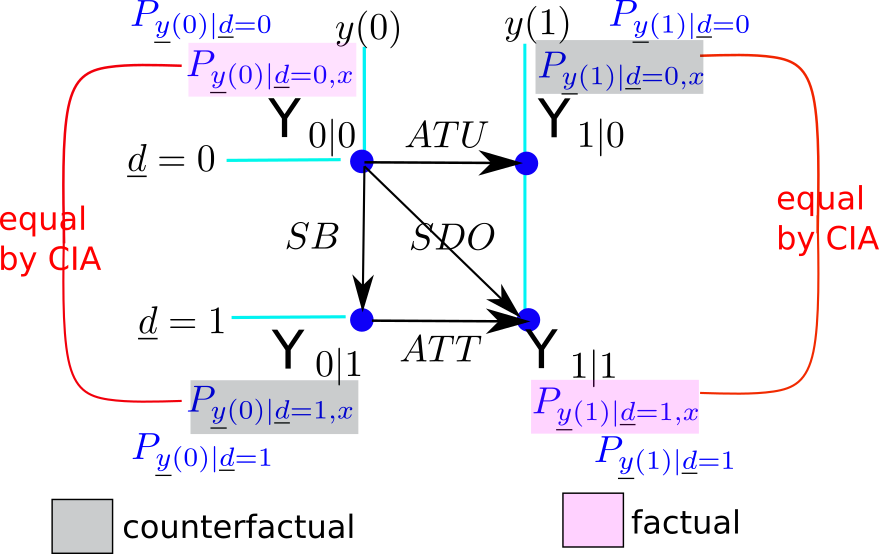
\includegraphics[width=4in]
{pot-out/y-diffs-square-probs.png}
\caption{Figure \ref{fig-y-diffs-square}
with added information
about  probability distributions
used to obtain each expected value
 $\caly_{c| d }$.}
\label{fig-y-diffs-square-probs}
\end{figure}


\begin{enumerate}
\item
Is it
possible for $SDO=0$ but $ATE\neq 0$
or vice versa, and
what is going on when this is true?
\item
What is going on when two treatment effects
are equal; for instance, when $ATT=ATU$?
\item
When is $\caly_{1|0}=\caly_{1}$,
and what is going on when this is  true?
\end{enumerate}
Fig.\ref{fig-y-diffs-square-probs}
gives some
intuition
about what is
going on when any of these
things happen.

Recall that
each expected value
$\caly_{c|d}$
is associated with a probability
distribution $P_{\rvy(c)|\rvd,x}$.

\beq
\caly_{c| d }
=
\sum_{y} y
\underbrace{\sum_x
P_{\rvy(c)| \rvd,x}(y| d,x)P(x|d)}_{
P_{\rvy(c)| \rvd}(y| d)}
\eeq
for $c,  d\in \bool$.
Fig.\ref{fig-y-diffs-square-probs}
reminds us of which $P$
is used to generate each $\caly$.
From this figure, we see that

\begin{enumerate}
\item
A sufficient
condition for $SDO=0$
is that
$P_{\rvy(1)| \rvd=1}
=
P_{\rvy(0)| \rvd=0}$.
A sufficient
condition for $ATE=0$
is that
$P_{\rvy(1)|x}
=
P_{\rvy(0)|x}$.

\item
A sufficient condition for
$ATT=ATU$
is that
$P_{\rvy(1)| \rvd=1,x}
-
P_{\rvy(0)| \rvd=1,x}$
equals
$P_{\rvy(1)| \rvd=0,x}
-
P_{\rvy(0)| \rvd=0,x}$.
\item
A sufficient condition for $\caly_{1|0}=\caly_{1}$
is that
$P_{\rvy(1)| \rvd=0}=
P_{\rvy(1)}$. Note that
the CIA implies that
$P_{\rvy(1)| \rvd=0,x}=
P_{\rvy(1)|x}$ always,
but this does not imply that
$P_{\rvy(1)| \rvd=0}=
P_{\rvy(1)}$.
\end{enumerate}


\section{$G_{do+}$  bnet}
\begin{figure}[h!]
$$
\begin{array}{ccccc}
\xymatrix{
&\rvx^\s\ar[dr]\ar[dl]
\\
\rvd^\s\ar[rr]&&\rvy^\s
}
&&
\xymatrix{
&\rvx^\s\ar[dr]
\\
\cald\rvd^\s=\td^\s\ar[rr]&&\rvy^\s
}
&&
\xymatrix{
&\rvx^\s\ar[dr]
\\
\cald\rvd^\s\ar[rr]&&\rvy^\s
}
\\
\\
G&&G_{do}= \cald_{\rvd^\s}
(\td^\s)G&& G_{do+}
\end{array}
$$
\caption{Bnet $G_{do}= \cald_{\rvd^\s}
(\td^\s)G$
is obtained by applying
the do operator to node $\rvd^\s$
of bnet $G$. Bnet $ G_{do+}$
is obtained
by adding a prior
probability distribution $P(\td^\s)$
to node $\cald\rvd^\s$ of
bnet $G_{do}$.}
\label{fig-po-G-do}
\end{figure}

Fig.\ref{fig-po-G-do}
shows how bnet $G_{do}$
is obtained by applying
the do operator to bnet $G$,
and
how
bnet $G_{do+}$
is obtained by adding
a prior
probability distribution
 to one of the nodes
of $G_{do}$.
In bnet $G_{do}$,
node  $\rvd^\s$ has been
stripped of all outside
influences and fixed to a
specific state $\td^\s$.
This is what an RCT does.

The TPMs, printed in blue,
for the bnets $G_{do}$
and $G_{do+}$,
are as follows.
Note that the TPMs
for bnets  $G_{do}$ and $G_{do+}$
are defined in terms
of the TPMs of bnet $G$.

\beq\color{blue}
P(x^\s)=
P_{\rvx}(x^\s)
\eeq

\beq
Q(\td)=\sum_x P_{\rvd|\rvx}
(\td|x)P_\rvx(x)
\eeq

\beq\color{blue}
P(\td^\s)=
\left\{
\begin{array}{ll}
\delta(\ul{\td^\s}, \td^\s)& \text{for $G_{do}$}
\\
Q(\td^\s)
& \text{for $G_{do+}$}
\end{array}
\right.
\eeq

\beq\color{blue}
P(y^\s|\td^\s, x^\s)=
P_{\rvy|\rvd, \rvx}(y^\s|\td^\s, x^\s)
\eeq

Note that in $G_{do}$,

\beq
P(\rvy=y|\cald \rvd=d, \rvx=x)=
P(y|\rvd=d,x)
\;
\label{eq-rho-begone}
\eeq
because, by the d-separation
theorem,  when we condition on
the confounder $\rvx$,
we  block information from being
transmitted from $\rvd$ to $\rvy$ through $\rvx$,
and this is equivalent to
amputating the arrow $\rvx\rarrow\rvd$.

Using Eq.(\ref{eq-rho-begone}), we get

\beqa
P(\rvy=y|\cald\rvd=d)
&=&
\sum_x
P(\rvy=y|\cald\rvd=d, x)P(x|\cald\rvd=d)
\\
&=&
\sum_x
P(y|d, x)P(x)
\label{eq-po-backdoor}
\eeqa
Eq.(\ref{eq-po-backdoor})
is called the {\bf backdoor adjustment formula}.
It allows us to
express a
probability
with a do operator
in its definition
in terms
of  probabilities
without do operators.

\section{$ACE=ATE$}


Define the Average
Causal Effect ($ACE$) by

\begin{align}
ACE&=\sum_y y
[P(y|\cald\rvd=1)-P(y|\cald\rvd=0)]
\\
&=
\sum_x P(x)\sum_y y [P(y|\rvd=1,x)-P(y|\rvd=0,x)]
\;. \text{ (by Eq.(\ref{eq-po-backdoor})}
\label{eq-my-backdoor-proof}
\end{align}


\begin{claim}\label{cl-ace-ate}
If we assume both SUTVA and
CIA (i.e., weak-d limit), then
\beq
ACE=ATE
\eeq
\end{claim}
\proof



\begin{align}
ACE&=
\sum_x P(x)\sum_y y [P(\rvy=y|\rvd=1,x)-
P(\rvy=y|\rvd=0,x)]
\\
&=\sum_x P(x)[\caly_{1|1, x}-\caly_{0|0, x}]
\;\text{(by SUTVA)}
\\
&=\sum_x P(x)[\caly_{1|x}-\caly_{0|x}]
\;\text{(by CIA)}
\\
&=
\caly_{1}-\caly_{0}
\\
&=
ATE
\end{align}
\qed

We will say there is a {\bf null result
in an RCT} when $ACE=0$. By the previous claim,
this is true iff $ATE=0$
(assuming weak-d limit).

\section{Good, Bad Controls}

The bnet $G_+$
of Fig.\ref{fig-po-G-im-y0-y1},
---the cornerstone of Rubin's
PO theory--- is limited in scope
and is easily
misapplied, leading
to incorrect results.
The problem is
some features
that are available
and could be conditioned on
shouldn't because they
would introduce spurious
contributions to ATE.
Such features are called
\qt{bad controls},
as opposed to \qt{good controls}\footnote{
In this section,
the word \qt{controls}
refers to the covariates
(i.e., independent
variables),
other than $\rvd$,
in a regression
with $\rvy$  as target
(i.e., independent)
variable.
This should
not be confused
with the
control
(i.e., untreated)
individuals
of a RCT.}
\footnote{An alternative to
the terms \qt{good and bad controls} is
\qt{good and bad strata}.}

Examples:

\hrule
\begin{enumerate}
\item
\begin{figure}[h!]
$$
\xymatrix{
*++[F-o]{\rvh_1} \ar[dd]\ar[dr]
&
& *++[F-o]{\rvh_2}  \ar[dd]\ar[dl]
\\
& \rvx
\\
\rvd \ar[rr]
&&\rvy
}$$
\caption{In this bnet,
$\rvx$ is a bad control
(i.e., should
not be conditioned on).
Nodes $\rvh_1$
and $\rvh_2$ are
hidden and therefore
cannot be conditioned on.}
\label{fig-po-m-bias}
\end{figure}

Consider the
bnet Fig.\ref{fig-po-m-bias},
which  Pearl calls M-bias,
because it looks like an M.
In that figure,
$\rvx$
is a \qt{bad control}
because
calculating
$ATE$ by conditioning on it,
and using the formula
$ATE=\sum_x
 P(x)[\caly_{1|x}-\caly_{0|x}]$,
yields a value of $ATE$
that is different from
$ACE$. This value for $ATE$
is unacceptable
because it does
not give the result of an RCT
whereas $ACE$ defined
in terms of do operators
always does.
The reason\footnote{We are
using here arguments
based on the d-separation
theorem
which is discussed in Chapter
\ref{ch-dsep}.} $ATE\neq ACE$
for this figure
is that in it,
$\rvx$ is
a collider node,
and conditioning
on it allows
rather than
prevents information
to flow from $\rvd$
to $\rvy$
via the path
$\rvd-\rvh_1-\rvx-\rvh_2-\rvy$.

\hrule
\item

\begin{figure}[h!]
$$
\xymatrix{
\rvc_1\ar[d]\ar[drr]
&&\rvc_2\ar@{<-->}[d]
\ar@{<-->}[dll]
\\
\rvd\ar[r]\ar[dr]
&\rvc_3\ar[r]
&\rvy\ar[dl]
\\
&\rvc_4
}$$
\caption{In this bnet,
node $\rvc_1$ is a good
control and nodes $\rvc_2, \rvc_3, \rvc_4$
are bad ones.}
\label{fig-po-1-good-3-bad}
\end{figure}

In Fig.\ref{fig-po-1-good-3-bad}, node
$\rvc_1$ is a good
control and nodes $\rvc_2, \rvc_3, \rvc_4$
are bad ones.

Conditioning on $\rvc_1$ blocks path $\rvd-\rvc_1-\rvy$, good

Conditioning on $\rvc_2$ opens path $\rvd-\rvc_2-\rvy$, bad

Conditioning on $\rvc_3$ blocks path $\rvd-\rvc_3-\rvy$, bad

Conditioning on $\rvc_4$ opens path $\rvd-\rvc_4-\rvy$, bad

\hrule
\item
(Taken from online course notes 
Ref.\cite{ethz-causality})

Consider the bnet

\beq
\xymatrix{
\rvx_2\ar[d]\ar[r]
&\rvx_3&
\rvx_4\ar[d]\ar[l]
\\
\rvd\ar[d]\ar[r]
&\rvx_6\ar[d]\ar[r]
&\rvy\ar[d]
&\rvx_7\ar[l]
\\
\rvx_8&\rvx_9&\rvx_{10}
}
\eeq
Find all  {\bf good strata (i.e., conditioning) sets} $\rvx.$ that block all
non-direct paths
 between $\rvd$ and $\rvy$.

Ans:
\begin{multicols}{4}
\begin{itemize}
\item $ \emptyset$
\item $\rvx_2$
\item $\rvx_4$
\item $\rvx_2, \rvx_4$
\item $\rvx_2,\rvx_3$
\item $\rvx_3, \rvx_4$
\item $\rvx_2, \rvx_3, \rvx_4$
\end{itemize}
\end{multicols}
Add $\rvx_7$
to each of the previous 7 possible
$\rvx.$. This gives
 a total of 14 possible
 conditioning sets. 
 For each of these conditioning sets $\rvx.$,
 we can write
 
 \beq
 P(y|\cald\rvd=d)=\sum_{x.}P(y|d, x.)P(x.)
 \eeq
 \hrule
\end{enumerate}

Pearl et al. have a paper
(Ref.\cite{pearl-good-neutral-bad})
that I highly recommend
that gives 20 examples
of good, neutral and
bad controls
in an $ATE$ calculation.
Those 20 examples are also analyzed
by my software SCuMpy (see Ref.\cite{scumpy}).

\section{PO Confounder Sensitivity Analysis}
\label{intro-pot-out-sensitivity}

There are various \qt{sensitivity analysis} strategies that are commonly
used
as a sanity check for a
PO analysis.
\begin{itemize}
\item {\bf vary columns of dataset}
\begin{enumerate}
\item {\bf randomize $\rvy$ column} (random outcome) This should make $ATE=0$.
\item {\bf randomize $\rvx$ column}
(random common cause) This should make $ATE=0$.
\item {\bf randomize $\rvd$ column} (placebo treatment dose) This should make $ATE=0$.
\item {\bf add new column $\rvu$}, where $\rvu$ is an \qt{unobserved
common cause}.
This should change $ATE$
in a predictable manner. See below.
\item {\bf add new column $\rvu$}, where $\rvu$ is a \qt{randomized
common cause}.
This should not change $ATE$.
\end{enumerate}
\item {\bf vary rows of dataset},
either all of them or some of them.
Replace them by a dataset that
should obey same DAG.
This should not change $ATE$.
\item {\bf vary good controls}. If using
a DAG that is more complicated than the
naive triangular PO DAG,
vary from one set of good
controls to another.
This should not change $ATE$.

\end{itemize}


\begin{figure}[h!]
$$
\begin{array}{cc}
\xymatrix{
\eps_\rvd\ar[ddd]
&\eps_\rvc\ar[d]
&\eps_\rvy\ar[ddd]
&\eps_\rvx\ar[lldd]
\\
&*++[F-o]{\rvc}\ar[ldd]_{\alp'}
\ar[rdd]^{\beta'}
\\
&\rvx
\ar[ld]^\alp
\ar[rd]_\beta
\\
\rvd\ar[rr]_\delta
&&\rvy
}
&
\xymatrix{
A_\rvc\eps_\rvd\ar[dd]
&A_\rvc\eps_\rvx\ar[d]
&A_\rvc\eps_\rvy\ar[dd]
\\
&A_\rvc\rvx
\ar[ld]^\alp
\ar[rd]_\beta
\\
A_\rvc\rvd\ar[rr]_\delta
&&A_\rvc\rvy
}
\\
(a)&(b)
\end{array}
$$
\caption{LDEN bnets used to do PO confounder
sensitivity analysis.
Node $\rvc$
is an unobserved common cause confounder.
The operator $A_\rvc$ in bnet $(b)$ annihilates $\rvc$ (i.e., $A_\rvc \rvc =0$)}
\label{eq-po-sen-ana}
\end{figure}

We end this section by
deriving a formula
for the change in $ATE$
when an unobserved
common cause $\rvc$ is added to the
naive triangular PO DAG.
(See Fig.\ref{eq-po-sen-ana})


Consider the LDEN bnet of Fig.\ref{eq-po-sen-ana} $(a)$,
whose structural equations,
printed in blue, are as follows:


\beq\color{blue}
\rvd=\alp\rvx +\alp'\rvc + \eps_\rvd
\eeq

\beq\color{blue}
\rvy = \beta \rvx + \beta'\rvc + \delta \rvd
+\eps_\rvy
\eeq
where $\eps_\rvd$ and $\eps_\rvy$
are root nodes with zero mean.
Therefore,

\beq
\rvc = \frac{1}{\alp'}(\rvd-\eps_\rvd -\alp\rvx)
\eeq

\beq
\rvy = \left(\beta-\;\frac{\alp\beta'}{\alp'}\right)\rvx
+\left(\delta+\frac{\beta'}{\alp'}\right)
\rvd-
\frac{\beta'}{\alp'}\eps_\rvd +\eps_\rvy
\eeq


\beq
\caly_{d|x,c}=E[\rvy(d)|x,c]=E[\rvy|d,x,c]
=\beta x+ \beta'c +\delta d
\eeq

\beq
\caly_{d|x}=E[\rvy(d)|x]=E[\rvy|d,x]=
\left(\beta-\;\frac{\alp\beta'}{\alp'}\right)x
+\left(\delta+\frac{\beta'}{\alp'}\right)
d
\eeq



\beq
ATE=E_x[ATE_x]=E_x[\caly_{1|x}-\caly_{0|x}]=
\delta+\frac{\beta'}{\alp'}
\eeq

\beq
ATE|_{\beta'=0}=\delta
\eeq

\beq
\boxed{
ATE-ATE|_{\beta'=0}=\frac{\beta'}{\alp'}}
\label{eq-po-ate-change}
\eeq
Note that the right-hand side
of Eq.(\ref{eq-po-ate-change})
is the product of the gains
along the path $\rvd\rarrow \rvc\rarrow\rvy$.
The gain
$1/\alp'$ for $\rvd\rarrow\rvc$
equals
the inverse of the gain
$\alp'$ for $\rvc\rarrow\rvd$.

Neither $\alp'$ nor $\beta'$
are observed, but the right-hand side
of Eq.(\ref{eq-po-ate-change})
can be bounded above by
an observed quantity.
This is done in Chapter \ref{ch-omitted-var-bias}.




\section{Strata-Matching}
\label{sec-strata-matching}

For a situation
described by
the bnet $G_{+}$
\ul{ in the weak-d limit},
we can match {\it similar}
individuals to fill the blank cells of
 Table \ref{tab-pot-out-missing}.
By \qt{similar}, we mean that
they have the same or almost the same
value of $\rvx^\s$.

The reason the weak-d limit
is required is that
it implies that $P(y(c)|d=0,x)=
P(y(c)|d=1,x)$ for $c\in \bool$,
Hence, we can sample from a
known factual $(c=d)$
distribution to
fill  the missing data
in the unknown counterfactual $(c\neq d)$
distribution.





\subsection{Exact   strata-matching}

\subsubsection{Estimates of Treatment Effects}
\label{sec-estimates}
For $ d\in \bool$ and all strata $x$,
define the sets of individuals
$A_{ d,x}=\{\s:  d^\s= d, x^\s=x\}$,
$A_x=A_{0,x}\cup A_{1,x}$ and $A=\cup_x A_x$.
Let $N_{ d,x}=|A_{ d,x}|$,
$N_x= |A_x|$ and $N=|A|$.

In exact   strata-matching,
we match each individual with
$ d^\s=d, x^\s=x$
with
exactly
one individual
with $ d^\s=1-d, x^\s=x$.
Define a map $m:A\rarrow A$
such that,
for each $x$, and
for $d\in \bool$,
if $\s\in A_{d,x}$, then
$m(\s)\in A_{1-d,x}$
This assumes $A_{0,x}$ and $A_{1,x}$
are non-empty for all $x$.
The purpose of map $m()$
is
to fill in the missing data in the
PO dataset. See Table \ref{tab-po-s-map}
for a pictorial representation of
this.

\begin{table}[h!]
\centering
\begin{tabular}{|l|l|l|}
\hline
 & \cellcolor[HTML]{ECF4FF}$y^\s(0)$ & \cellcolor[HTML]{ECF4FF}$y^\s(1)$ \\ \hline
\cellcolor[HTML]{ECF4FF}$ d^\s=0$ & $y^\s$ & $y^{m(\s)}$ \\ \hline
\cellcolor[HTML]{ECF4FF}$ d^\s=1$ & $y^{m(\s)}$ & $y^\s$ \\ \hline
\end{tabular}
\caption{Illustration of the
purpose of the map $m()$.
Note that $y^\s=y^\s( d^\s)$
 and $y^{m(\s)}=y^\s(1-d^\s)$.}
\label{tab-po-s-map}
\end{table}



Note that
\beq
\sum_{\s\in A_{x}}\frac{d^\s}{N_{1,x}}=
\sum_{\s\in A_{1,x}}\frac{1}{N_{1,x}}=1
\;.
\eeq
Thus

\beq
\sum_{\s\in A_{x}}\frac{d^\s}{N_{1,x}}y^\s=
E_{\s| d=1,x}[y^\s]=\caly_{1|1,x}
\eeq
Table \ref{tab-po-yc-at-dx}
gives
estimates of
$ \caly_{c| d ,x}$

{\renewcommand{\arraystretch}{1.5}
\begin{table}[h!]
\centering
\begin{tabular}{|l|l|l|}
\hline
 & \cellcolor[HTML]{ECF4FF}$y^\s(0)$
& \cellcolor[HTML]{ECF4FF}$y^\s(1)$
\\ \hline
\cellcolor[HTML]{ECF4FF}$ d^\s=0$
&
$\frac{1}{N_{0,x}}\sum_{\s\in A_x} (1- d^\s)y^{\s}=\caly_{0|0,x}$
&
$\frac{1}{N_{0,x}}\sum_{\s\in A_x} (1- d^\s) y^{m(\s)}=\caly_{1|0,x}$
\\ \hline
\cellcolor[HTML]{ECF4FF}$ d^\s=1$
&
 $\frac{1}{N_{1,x}}\sum_{\s\in A_x}  d^\s y^{m(\s)}=\caly_{0|1,x}$
&
$\frac{1}{N_{1,x}}\sum_{\s\in A_x}  d^\s y^\s=\caly_{1|1,x}$
\\ \hline
\end{tabular}
\caption{Estimates of
$ \caly_{c| d ,x}$.}
\label{tab-po-yc-at-dx}
\end{table}}

{\renewcommand{\arraystretch}{1.5}
\begin{table}[h!]
\centering
\begin{tabular}{|l|l|l|}
\hline
 & \cellcolor[HTML]{ECF4FF}$y^\s(0)$
& \cellcolor[HTML]{ECF4FF}$y^\s(1)$
\\ \hline
\cellcolor[HTML]{ECF4FF}$ d^\s=0$
&
$\frac{1}{N_{x}}\sum_{\s\in A_x}
(1- d^\s)y^{\s}=\caly_{0,0|x}$
&
$\frac{1}{N_{x}}\sum_{\s\in A_x}
 (1- d^\s) y^{m(\s)}=\caly_{1,0|x}$
\\ \hline
\cellcolor[HTML]{ECF4FF}$ d^\s=1$
&
 $\frac{1}{N_{x}}\sum_{\s\in A_x}
 d^\s y^{m(\s)}=\caly_{0,1|x}$
&
$\frac{1}{N_{x}}\sum_{\s\in A_x}
 d^\s y^\s=\caly_{1,1|x}$
\\ \hline
\end{tabular}
\caption{Estimates of
$ \caly_{c, d| x}$.}
\label{tab-po-ycd-at-x}
\end{table}}


Recall that

\beq
\caly_{c,d|x}=\caly_{c|d,x}P(d|x)
\eeq
Hence,

\beqa
\caly_{c,d|x}
&=&
(N_{d,x}\caly_{c|d,x})
\frac{P(d|x)}{N_{d,x}}
\\
&=&
(N_{d,x}\caly_{c|d,x})
\frac{1}{N_x}
\eeqa
Table \ref{tab-po-ycd-at-x}
gives
estimates of
$ \caly_{c, d |x}$


The treatment effects $\cale\in
\{ATE, ATT, ATU, SB, SDO\}$
can be estimated from the data
via the following estimates.



\beqa
\HAT{ATE}_x
&=&
\overbrace{
\caly_{1|1,x}P(1|x) +
 \caly_{1|0,x}P(0|x)}^
{\caly_{1|x}}
-
\overbrace{(
\caly_{0|1,x}P(1|x) +
\caly_{0|0,x}P(0|x))}^
{\caly_{0|x}}
\\
&=&
\frac{1}{N_x}[
\HAT{ATT}_x N_{1,x} +
\HAT{ATU}_x N_{0,x}]
\\
&=&
\frac{1}{N_x}
\left[\sum_{\s\in A_x}  d^\s [y^\s - y^{m(\s)}]+
\sum_{\s\in A_x}(1- d^\s) [ y^{m(\s)}-y^\s]
\right]
\\
&=&
\frac{1}{N_x}\sum_{\s\in A_x} (2 d^\s-1)[y^\s -y^{m(\s)}]
\label{eq-est-ate}
\eeqa

\beqa
\HAT{ATT}_x
&=&
\overbrace{\frac{1}{N_{x}}
\sum_{\s\in A_x}  d^\s y^\s}
^{\caly_{1,1|x}}
 -
\overbrace{\frac{1}{N_{x}}
\sum_{\s\in A_x}  d^\s y^{m(\s)}}
^{\caly_{0,1|x}}
\\
&=&
\frac{1}{N_{x}}\sum_{\s\in A_x}
 d^\s [y^\s - y^{m(\s)}]
\label{eq-est-att}
\eeqa


\beqa
\HAT{ATU}_x
&=&
\overbrace{\frac{1}{N_{x}}
\sum_{\s\in A_x} (1- d^\s) y^{m(\s)} }
^{\caly_{1,0|x}}
 -
\overbrace{\frac{1}{N_{x}}
\sum_{\s\in A_x} (1- d^\s)y^\s}
^{\caly_{0,0|x}}
\\
&=&
\frac{1}{N_{x}}\sum_{\s\in A_x} (1- d^\s) [ y^{m(\s)}-y^\s]
\label{eq-est-atu}
\eeqa

\beq
\HAT{SB}_x =
\overbrace{\frac{1}{N_{x}}
\sum_{\s\in A_x}  d^\s y^{m(\s)}}
^{\caly_{0,1|x}}
-
\overbrace{\frac{1}{N_{x}}
\sum_{\s\in A_x} (1- d^\s)y^\s}
^{\caly_{0,0|x}}
\label{eq-est-sb}
\eeq

\beq
\HAT{SDO}_x=
\overbrace{\frac{1}{N_{x}}
\sum_{\s\in A_x}  d^\s y^\s}^
{\caly_{1,1|x}}
-
\overbrace{\frac{1}{N_{x}}
\sum_{\s\in A_x} (1- d^\s) y^\s}^
{\caly_{0,0|x}}
\label{eq-est-sdo}
\eeq



Suppose we do linear regression
to fit a
hyperplane $y(x)$ to
the dataset set $\{(x^\s, y^\s):\s\}$,
and then we calculate
$\pder{\rvy}{\rvd}=\delta$.
Out
of all
the treatment effects,
this $\delta$ is
probably (?) closest
to $ACE=ATE$.
Note also that the
linear regression
method
of estimating
$\delta$
does imputation
(guesses missing values)
by doing a linear fit.
One can also
use machine learning to
do a non-linear fit.
In contrast, the estimates
of treatment effects
presented in this section
do imputation by
non-linear  strata-matching.

\subsubsection{Example, estimation of treatment effects}


For $\s\in \{1,2, \ldots, 10\}$, define

\beq
m(\s)=
\left\{
\begin{array}{ll}
\s+5&\text{if }\s\leq 5
\\
\s-5&\text{if }\s >5
\end{array}
\right.
\eeq


{\renewcommand{\arraystretch}{1.5}
\begin{table}[h!]
\centering
\begin{tabular}{|l|l|l|l|l|l|l|}
\hline
\cellcolor[HTML]{ECF4FF} $\s$& \cellcolor[HTML]{ECF4FF}$ d^\s$ & \cellcolor[HTML]{ECF4FF}$y^\s$ & \cellcolor[HTML]{ECF4FF}$ d^\s y^\s$ & \cellcolor[HTML]{ECF4FF}$(1- d^\s)y^\s$ & \cellcolor[HTML]{ECF4FF}$ d^\s y^{m(\s)}$ & \cellcolor[HTML]{ECF4FF}$(1- d^\s)y^{m(\s)}$ \\ \hline
\cellcolor[HTML]{ECF4FF}1 & \cellcolor[HTML]{FFFFC7}0 & 0 & \cellcolor[HTML]{FFFFC7}0 & 0 & \cellcolor[HTML]{FFFFC7}0 & 0 \\ \hline
\cellcolor[HTML]{ECF4FF}2 & \cellcolor[HTML]{FFFFC7}0 & 0 & \cellcolor[HTML]{FFFFC7}0 & 0 & \cellcolor[HTML]{FFFFC7}0 & 1 \\ \hline
\cellcolor[HTML]{ECF4FF}3 & \cellcolor[HTML]{FFFFC7}0 & 1 & \cellcolor[HTML]{FFFFC7}0 & 1 & \cellcolor[HTML]{FFFFC7}0 & 1 \\ \hline
\cellcolor[HTML]{ECF4FF}4 & \cellcolor[HTML]{FFFFC7}0 & 1 & \cellcolor[HTML]{FFFFC7}0 & 1 & \cellcolor[HTML]{FFFFC7}0 & 1 \\ \hline
\cellcolor[HTML]{ECF4FF}5 & \cellcolor[HTML]{FFFFC7}0 & 1 & \cellcolor[HTML]{FFFFC7}0 & 1 & \cellcolor[HTML]{FFFFC7}0 & 1 \\ \hline
\cellcolor[HTML]{ECF4FF}6 & 1 & 0 & 0 & \cellcolor[HTML]{FFFFC7}0 & 0 & \cellcolor[HTML]{FFFFC7}0 \\ \hline
\cellcolor[HTML]{ECF4FF}7 & 1 & 1 & 1 & \cellcolor[HTML]{FFFFC7}0 & 0 & \cellcolor[HTML]{FFFFC7}0 \\ \hline
\cellcolor[HTML]{ECF4FF}8 & 1 & 1 & 1 & \cellcolor[HTML]{FFFFC7}0 & 1 & \cellcolor[HTML]{FFFFC7}0 \\ \hline
\cellcolor[HTML]{ECF4FF}9 & 1 & 1 & 1 & \cellcolor[HTML]{FFFFC7}0 & 1 & \cellcolor[HTML]{FFFFC7}0 \\ \hline
\cellcolor[HTML]{ECF4FF}10 & 1 & 1 & 1 & \cellcolor[HTML]{FFFFC7}0 & 1 & \cellcolor[HTML]{FFFFC7}0 \\ \hline
\end{tabular}
\caption{Estimates of treatment effects
are calculated for this example. }
\label{tab-po-example}
\end{table}
}


\begin{table}[h!]
\centering
\begin{tabular}{|
>{\columncolor[HTML]{ECF4FF}}l |l|l|}
\hline
\cellcolor[HTML]{CBCEFB}$N( d, y)$ & \cellcolor[HTML]{ECF4FF}$y=0$ & \cellcolor[HTML]{ECF4FF}$y=1$ \\ \hline
$ d=0$ & 2 & 3 \\ \hline
$ d=1$ & 1 & 4 \\ \hline
\end{tabular}
\caption{$N(\ul{ d^\s}=d, \rvy^\s=y)$ for
the data in Table \ref{tab-po-example}.}
\label{tab-n-po-example}
\end{table}

Let $N(\cals)$
be the number of individuals $\s$
that satisfy condition $\cals$.
For example,
$N(\ul{ d^\s}= d)$
is the number of individuals
such that $\ul{ d^\s}= d$.

\beq
N_1
=
N( d^\s=1)
=
5
\eeq

\beq
N_0
=
N( d^\s=0)
=
5
\eeq

\beq
N
= N_0+N_1
=
10
\eeq



\beq
\caly_{1|1}
=
\frac{1}{N_1}
\sum_\s  d^\s y^\s
=
\frac{4}{5}
\eeq

\beq
\caly_{0|0}
=
\frac{1}{N_0}
\sum_\s (1- d^\s) y^\s
=
\frac{3}{5}
\eeq

\beq
\caly_{0|1}
=
\frac{1}{N_1}
\sum_\s  d^\s y^{m(\s)}
=
\frac{3}{5}
\eeq

\beq
\caly_{1|0}
=
\frac{1}{N_0}
\sum_\s (1- d^\s) y^{m(\s)}
=
\frac{4}{5}
\eeq

\beq
ATT=
\caly_{1|1}-\caly_{0|1}
=\frac{1}{5}
\eeq

\beq
ATE=ATT=ATU=SDO=\frac{1}{5}
\;,\;\; SB=0
\label{eq-all-equal}
\eeq

This example is unusual
in that it has a single
stratum $x$, and for
that stratum,
the treated and
untreated populations
are {\bf balanced} (of equal size).
Also, the map $m()$
is 1-1 onto.
If, for instance,
$m(\s)=6$ for all $\s\in A_0$
and $m(\s)=5$ for $\s\in A_1$,
then $ATE, ATT, ATU, SDO$
would not all be same, and
$SB$ would not be zero.
In fact, whenever there is a single
balanced stratum and the map $m()$
is 1-1 onto, Eq.(\ref{eq-all-equal})
can be proven to be true using
the methods of
section \ref{sec-td-ignored}.


\subsection{Approximate   strata-matching}

It is very often
the case that
one can't
find for a given
individual $\s$
another individual that has
opposite $ d^\s$ but
exactly the same value of $x^\s$.
In such cases, one can discard all
matchless individuals.
But that would entail a loss
of precious information.
Instead of discarding orphans,
a better way is to
relax our demands and
match individual $\s$
with another individual $m(\s)$
such that $x^\s$
and $x^{m(\s)}$ are very
close in some metric.
Alternatively, the matching
individual might
not be real; it might
be a composite
of individuals.

More precisely,
for some arbitrary
parameter $\eps>0$,
and an individual $\s$,
define
the {\bf  strata-matching set}
$\calm_{\eps}(\s)$ by\footnote{
One can use an $\eps$
that depends on $\s$.
For example, let $\eps(\s, 5)$
satisfy
$|\calm_{\eps(\s, 5)}(\s)|=5$.}

\beq
\calm_{\eps}(\s)=
\{m:  d^m=1-d^\s,
dist(x^\s, x^m)\leq \eps \}
\;,
\eeq
where

\beq
dist(x^\s, x^m)=
[x^\s]^T [\Sigma]^{-1} x^m
\;,
\eeq
where $\Sigma = \av{\rvx^\s, [\rvx^m]^T}$.
 This
metric $dist(x^\s, x^m)$ is
called the {\bf Mahalanobis distance}.
We will call
the case $\eps=0$ an {\bf  exact   strata-matching},
and
the case
$\eps\neq 0$
 an {\bf approximate   strata-matching.}.
To do an approximate   strata-matching,
replace $y^{m(\s)}$
by
$\av{y}^{\calm_\eps(\s)}$
in
the estimates
given above
for an exact   strata-matching.
$\av{y}^{\calm_\eps(\s)}$
is defined by

\beq
\av{y}^{\calm_\eps(\s)}=
\frac{1}{|\calm_{\eps}(\s)|}
\sum_{m\in \calm_{\eps}(\s)}
y^m
\;.
\eeq

\subsection{Unbiased  strata-matching
estimates}
The estimates we obtained
via  strata-matching
are biased
because  strata-matching,
due to its non-uniqueness,
 introduces
noise into the estimate. However,
one can define new
bias-corrected estimates.
Following Ref.\cite{book-mixtape},
we will
next
find an unbiased estimate
of
$ATT_x$
using the biased estimate
of
$ATT_x$ that we
obtained by  strata-matching.



Let $\HAT{\caly}_{|d, x}$
be an estimate
of $\caly_{|d, x}
=E_{|d,x}[\rvy]$
that is
obtained, for
example, via
 Linear Regression.

\begin{claim}
The quantity

\beq
\HAT{ATT}_x^{unbi}=
\frac{1}{N_x}
\sum_{\s\in A_x}d^\s
\left[
(y^\s-y^{m(\s)})
-(\HAT{\caly}_{|0, x^\s}-
\HAT{\caly}_{|0, x^{m(\s)}})
\right]
\;
\eeq
is an unbiased estimate of $ATT_x$.
\end{claim}
\proof

We begin by assuming
a special case of
SUTVA. Let

\beq
\rvy^\s=\rvy(d^\s)=
\HAT
{\caly}_{|d^\s,x^\s} + \ul{\eps}^\s
\eeq
where

\beq
\av{\HAT
{\caly}_{|d^\s,x^\s},\ul{\eps}^\s
}_\s=0
\eeq

Recall that the biased estimate
of $ATT_x$ obtained by strata-matching is

\beq
\HAT{ATT}_x^{bi}=
\frac{1}{N_x}
\sum _{\s\in A_x}
d^\s(y^\s-y^{m(\s)})
\eeq
where $\s$ and $m(\s)$
are matched (i.e.,
$x^\s\approx x^{m(\s)}$
and $d^{m(\s)}=1-d^\s$).

\beqa
\HAT{ATT}_x^{bi}
&=&
\frac{1}{N_x}
\sum _{\s\in A_x}
d^\s\left(
\HAT{\caly}_{|1,x^\s}
-
\HAT{\caly}_{|0,x^{m(\s)}}
\right)
\\
&+&
\frac{1}{N_x}
\sum _{\s\in A_x}
d^\s(\eps^\s-\eps^{m(\s)})
\eeqa

\beqa
\HAT{ATT}_x^{bi}
&=&
\underbrace{
\frac{1}{N_x}
\sum _{\s\in A_x}
d^\s\left(
\HAT
{\caly}_{|1,x^\s}
-
\HAT
{\caly}_{|0,x^\s}
\right)
}_{ {ATT_x}^{unbi}}
\\
&+&
\underbrace{
\frac{1}{N_x}
\sum _{\s\in A_x}
d^\s\left(
\HAT
{\caly}_{|0,x^\s}
-
\HAT
{\caly}_{|0,x^{m(\s)}}
\right)
}_{\Delta ATT_x}
\\
&+&
\underbrace{
\frac{1}{N_x}
\sum _{\s\in A_x}
d^\s(\eps^\s-\eps^{m(\s)})
}_{\cale_x}
\eeqa

\beq
{ATT_x}^{unbi}
=
\underbrace{\HAT{ATT}_x^{bi}
- \Delta ATT_x}_{
\HAT{ATT}_x^{unbi}}
-\cale_x
\eeq

By the Central
Limit Theorem,
for large $N_x$,
this sum over $\s\in A_x$
of i.i.d. variables
is normally
distributed

\beq
\sqrt {N_x}
{ATT}^{unbi}_x
\sim \caln(x; 0, var)
\eeq
The reason for
the $\sqrt{N_x}$
normalization
is that we want the variance
to be proportional
to $N_x$.

\beqa
var &=& N_x
\av{{ATT}^{unbi}_x,
{ATT}^{unbi}_x}
\\
&=&
N_x\av{\HAT{ATT}_x^{unbi},
\HAT{ATT}_x^{unbi}}
+
N_x\av{\cale_x, \cale_x}
\eeqa
\qed

\section{$(SDO,ATE)$ space}
If we substitute
$y^\s\rarrow y^\s( d^\s)$ and
 $y^{m(\s)}\rarrow y^\s(1-d^\s)$
into
the estimate
Eq.(\ref{eq-est-ate}) for $ATE$
and the estimate
Eq.(\ref{eq-est-sdo}) for $SDO$,
we get

\beqa
\HAT{ATE}_x
&=&
\frac{1}{N_x}\sum_{\s\in A_x}
 (2 d^\s-1)[y^\s( d^\s) -y^\s(1-d^\s)]
\\
&=&
\frac{1}{N_x}\sum_{\s\in A_x}
 [y^\s(1) -y^\s(0)]
\label{eq-est-ate-simple}
\eeqa
and

\beqa
\HAT{SDO}_x
&=&
\frac{1}{N_{1,x}}
\sum_{\s\in A_x}  d^\s y^\s( d^\s)
-
\frac{1}{N_{0,x}}
\sum_{\s\in A_x} (1- d^\s) y^\s( d^\s)
\\
&=&
\frac{1}{N_{1,x}}
\sum_{\s\in A_{1,x}} y^\s(1)
-
\frac{1}{N_{0,x}}
\sum_{\s\in A_{0,x}}  y^\s(0)
\;.
\label{eq-est-sdo-simple}
\eeqa

Recall that
$\HAT{\cale}=E_x[\HAT{\cale}_x]=
\sum_x \frac{N_x}{N}\HAT{\cale}_x$
for $\cale\in\{ATE, SDO\}$.

Recall also that
$ACE=ATE=0$ is the null
result in an RCT.


Suppose that
the treatment outcome $y^\s$
has only two
possible values, 0 and 1.
Then, $-1\leq ATE \leq 1$
and
$-1\leq SDO \leq 1$.
But does  $ATE=0$
imply $SDO=0$
or vice versa?
Next, we answer
that question
and more
by finding
the region
of accessibility in the
$(SDO, ATE)$
plane,
assuming $y^\s\in \bool$.


\newpage

\begin{figure}[h!]
\centering
\subfloat[$ATE=-1$ $(SDO=-1)$ point A]{
\begin{tabular}{|
>{\columncolor[HTML]{ECF4FF}}l |l|l|l|}
\hline
\cellcolor[HTML]{CBCEFB}$\s$ & \cellcolor[HTML]{CBCEFB}$ d^\s$ & \cellcolor[HTML]{CBCEFB}$y^\s(0)$ & \cellcolor[HTML]{CBCEFB}$y^\s(1)$ \\ \hline
1 & 0 & 1 & 0 \\ \hline
2 & 0 & 1 & 0 \\ \hline
3 & 0 & 1 & 0 \\ \hline
4 & 1 & 1 & 0 \\ \hline
5 & 1 & 1 & 0 \\ \hline
6 & 1 & 1 & 0 \\ \hline
\end{tabular}
}
\quad
\subfloat[$ATE=\frac{1}{2}$ $(SDO=0)$ point B]{
\begin{tabular}{|
>{\columncolor[HTML]{ECF4FF}}l |l|l|l|}
\hline
\cellcolor[HTML]{CBCEFB}$\s$ & \cellcolor[HTML]{CBCEFB}$ d^\s$ & \cellcolor[HTML]{CBCEFB}$y^\s(0)$ & \cellcolor[HTML]{CBCEFB}$y^\s(1)$ \\ \hline
1 & 0 & 0 & 1 \\ \hline
2 & 0 & 0 & 1 \\ \hline
3 & 0 & 0 & 1 \\ \hline
4 & 1 & 0 & 0 \\ \hline
5 & 1 & 0 & 0 \\ \hline
6 & 1 & 0 & 0 \\ \hline
\end{tabular}
}
\quad
\subfloat[$ATE=1$ $(SDO=1$) point C]{
\begin{tabular}{|
>{\columncolor[HTML]{ECF4FF}}l |l|l|l|}
\hline
\cellcolor[HTML]{CBCEFB}$\s$ & \cellcolor[HTML]{CBCEFB}$ d^\s$ & \cellcolor[HTML]{CBCEFB}$y^\s(0)$ & \cellcolor[HTML]{CBCEFB}$y^\s(1)$ \\ \hline
1 & 0 & 0 & 1 \\ \hline
2 & 0 & 0 & 1 \\ \hline
3 & 0 & 0 & 1 \\ \hline
4 & 1 & 0 & 1 \\ \hline
5 & 1 & 0 & 1 \\ \hline
6 & 1 & 0 & 1 \\ \hline
\end{tabular}
}
\caption{Examples of PO datasets. Exploring $ATE$ extremes.}
\label{fig-ate-possi}
\end{figure}

\begin{figure}[h!]
\centering
\subfloat[$SDO=-1$ $(ATE=0)$ point D]{
\begin{tabular}{|
>{\columncolor[HTML]{ECF4FF}}l |l|l|l|}
\hline
\cellcolor[HTML]{CBCEFB}$\s$ & \cellcolor[HTML]{CBCEFB}$ d^\s$ & \cellcolor[HTML]{CBCEFB}$y^\s(0)$ & \cellcolor[HTML]{CBCEFB}$y^\s(1)$ \\ \hline
1 & 0 & 1 & 1 \\ \hline
2 & 0 & 1 & 1 \\ \hline
3 & 0 & 1 & 1 \\ \hline
4 & 1 & 0 & 0 \\ \hline
5 & 1 & 0 & 0 \\ \hline
6 & 1 & 0 & 0 \\ \hline
\end{tabular}
}
\quad
\subfloat[$SDO=0$ $(ATE=-\;\frac{1}{2})$ point E]{
\begin{tabular}{|
>{\columncolor[HTML]{ECF4FF}}l |l|l|l|}
\hline
\cellcolor[HTML]{CBCEFB}$\s$ & \cellcolor[HTML]{CBCEFB}$ d^\s$ & \cellcolor[HTML]{CBCEFB}$y^\s(0)$ & \cellcolor[HTML]{CBCEFB}$y^\s(1)$ \\ \hline
1 & 0 & 1 & 0 \\ \hline
2 & 0 & 1 & 0 \\ \hline
3 & 0 & 1 & 0 \\ \hline
4 & 1 & 1 & 1 \\ \hline
5 & 1 & 1 & 1 \\ \hline
6 & 1 & 1 & 1 \\ \hline
\end{tabular}
}
\quad
\subfloat[$SDO=1$ $(ATE=0$) point F]{
\begin{tabular}{|
>{\columncolor[HTML]{ECF4FF}}l |l|l|l|}
\hline
\cellcolor[HTML]{CBCEFB}$\s$ & \cellcolor[HTML]{CBCEFB}$ d^\s$ & \cellcolor[HTML]{CBCEFB}$y^\s(0)$ & \cellcolor[HTML]{CBCEFB}$y^\s(1)$ \\ \hline
1 & 0 & 0 & 0 \\ \hline
2 & 0 & 0 & 0 \\ \hline
3 & 0 & 0 & 0 \\ \hline
4 & 1 & 1 & 1 \\ \hline
5 & 1 & 1 & 1 \\ \hline
6 & 1 & 1 & 1 \\ \hline
\end{tabular}
}
\caption{Examples of PO datasets. Exploring $SDO$ extremes.}
\label{fig-sdo-possi}
\end{figure}

\begin{figure}[h!]
\centering
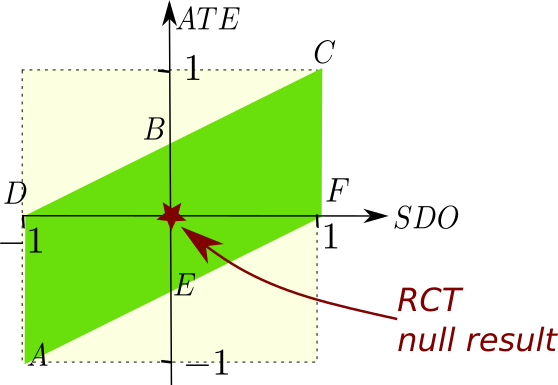
\includegraphics[width=2.5in]
{pot-out/sdo-ate-polytope.png}
\caption{
Green parallelogram
is accessible region in
$(SDO,ATE)$ plane,
assuming $y^\s\in \bool$.
Each of the
six points A, B, \ldots F
corresponds to one of the six tables
in Figs. \ref{fig-ate-possi}
and \ref{fig-sdo-possi}.
Segment $DF$
corresponds to the null
result in an RCT.
}
\label{fig-sdo-ate-polytope}
\end{figure}




\section{Propensities}\label{sec-propensities}

It is often the case
that the discrete vector $\rvx^\s$
has
too many possible values to make
matching possible.
In such cases, it
is convenient to
map the space
of vectors
$\rvx^\s$
to the real line.
One very
convenient choice
for that map
is the
{\bf propensity score},
which is defined as

\beq
g(x^\s)=P(\rvd^\s=1|x^\s)
\;.
\eeq
$P(\rvd^\s=1|x^\s)$ is easy to calculate
from the dataset, using $g(x)=N_{1,x}/N_x$.

\begin{figure}[h!]
$$
\begin{array}{ccc}
\xymatrix@C=.8pc{
&&\rvx^\s\ar[ddll]\ar[d]
\\
&&[\rvy^\s(0),\rvy^\s(1)]\ar[d]
\\
\rvd^\s\ar[urr]^?\ar[rr]
&
&\rvy^\s
}
&
\xymatrix@C=.8pc{
&&\rvx^\s\ar[dl]\ar[d]
\\
&\rvg^\s\ar[dl]
&[\rvy^\s(0),\rvy^\s(1)]\ar[d]
\\
\rvd^\s\ar[urr]^?\ar[rr]
&
&\rvy^\s
}
&
\xymatrix@C=.8pc{
&&\rvg^\s\ar[ddll]\ar[d]
\\
&&[\rvy^\s(0),\rvy^\s(1)]\ar[d]
\\
\rvd^\s\ar[urr]^?\ar[rr]
&
&\rvy^\s
}
\\
G_+&G_{g1}&G_{g2}
\end{array}
$$
\caption{Bnets $G_+, G_{g1}, G_{g2}$
used when doing propensity scoring.}
\label{fig-po-G-ps}
\end{figure}
To use the
propensity score,
one replaces the bnet $G_{+}$
by the bnet $G_{g1}$ as
shown in Fig.\ref{fig-po-G-ps}.
The TPMs, printed in blue,
for the 2 nodes of $G_{g1}$
that differ from the nodes
of $G_{+}$,
are as follows:\footnote{$g$ is a continuous variable
in the interval $[0,1]$
so its distribution
$P(g|x)$ is a Dirac delta function. }


\beq\color{blue}
P(g^\s|x^\s)=
\delta(g^\s-g(x^\s))
\eeq

\beq\color{blue}
P(d^\s|g^\s)=
g^\s d^\s + (1-g^\s)(1-d^\s)
\eeq

Note that
these TPMs are self-consistent because

\beqa
P(d|x)&=&
\sum_g P(d|g)P(g|x)
\\
&=&
g(x)d + [1-g(x)](1-d)
\\
&=&
\left\{
\begin{array}{ll}
g(x)&\text{if }d=1
\\
1-g(x) & \text{if }d=0
\end{array}
\right.
\\
&=&
P(d|x)
\eeqa


We would like to do
{\bf propensity score strata-matching} by
matching g-strata instead of x-strata.
To do g-strata-matching,
we use the graph $G_{g2}$
in Fig.\ref{fig-po-G-ps}
which differs from graph $G_+$
in that node $\rvx^\s$ is replaced
by node $\rvg^\s$.
Next we get the TPM of graph $G_{g2}$
in terms of the TPM of graph $G_+$.
We do this by expressing
$P(d|g)$, $P(g)$
and $P(y|d,g)$
in terms of
$P(d|x)$, $P(x)$
and $P(y|d,x)$.

From the TPMs
for $G_{g1}$, one has

\beq
\boxed{
P(d|g)=
g d + (1-g)(1-d)}
\eeq
and

\beq
\boxed{
P(g)=\sum_x \overbrace{
\delta(g-g(x))}^{P(g|x)}
P(x)}
\;.
\eeq
Note that $P(g)$ is a linear
combination of Dirac delta functions.
Next, note that


\beq
P(y| d,g)=
\sum_x P(y|d,x)P(x|g)
\eeq
so we need to find $P(x|g)$. Since

\beqa
P(x|g)&=&\frac{P(g|x)P(x)}{P(g)}
\\
&=&
\frac{\delta(g-g(x))P(x)}{P(g)}
\eeqa
we finally get

\beq
\boxed{
P(y| d,g)=
\sum_x P(y|d,x)
\frac{\delta(g-g(x))P(x)}{P(g)}
}
\;.
\label{eq-p-y-dg}
\eeq

Eq.(\ref{eq-p-y-dg})
looks complicated, but all
it is saying is that

\beq
P(y|d,g)P(g)= N_g
\sum_{x\in g^{-1}(g)}
 P(y|d,x)P(x)
\;,
\eeq
where $g^{-1}(g)=
\{x: g(x)=g\}$
and $N_g$ is the number of $g$
when we discretize the interval $[0,1]$.
In general,

\beq
\sum_x\delta(g-g(x))= N_g
\sum_{x\in g^{-1}(g)}
\eeq



Recall that for any treatment
effect $\cale
\in \{ATE, ATT,ATU, SB, SDO\}$,
we can estimate $\cale_x$,
and then calculate $\cale$ from it, using
\beq
\cale
=
\sum_x P(x) \cale_x
\eeq
In terms of $g$, this becomes
\beq
\cale = \int_0^1 dg \;P(g) \cale_{x\rarrow g}
\eeq
If we smooth $P(g)$, then the
 integral over $g$ can be done by complex contour integration and reduces to a finite sum over a few residues.
The large sum over $x$ has been
swept under the rug, into the calculation of $P(g)$.

\subsection{Propensity based  estimates of
Treatment Effects}

In the  strata-matching
section \ref{sec-strata-matching}, we gave an estimate
of $ACE_x$.
In strata-matching, one
fills in the missing
counterfactual values
via the map $m()$.
This is justified
because,
by CIA (weak-d limit),
the counterfactual
distributions
are assumed to equal
the factual distributions (see Fig.
\ref{fig-y-diffs-square-probs}).
In this
section,
we give estimates
of treatment effects that
are based on the  formulae derived
in Section \ref{sec-propensities}.
The estimates given in this section
do not require
the map $m()$, because
the identification of
counterfactual distributions
with factual ones was used to
derive the formulae
of  Section \ref{sec-propensities}.

Let
\beq
g_{d|x}=g_d(x)=P(d|x)
\eeq
 for $d\in\bool$.
Note that $g_{0|x}+g_{1|x}=1$.
We will
refer to $g_d(x)$
for $d\in \bool$
as {\bf dual propensities}
and to $g_1(x)$ as the
{\bf propensity score}.

Define
\beq
\delta_{y|x}=
P(y|\rvd=1,x)-P(y|\rvd=0,x)
\eeq
Note that

\beqa
\delta_{y|x}
&=&
\frac{P(y, \rvd=1|x)}{g_{1|x}}
-
\frac{P(y, \rvd=0| x)}{g_{0|x}}
\\
&=&
\frac{P(y, \rvd=1|x)g_{0|x}
-
P(y, \rvd=0|x)g_{1|x}}
{
g_{0|x}g_{1|x}
}
\\
&=&
\frac{P(y, \rvd=1|x)
-
P(y|x)g(x)}
{
g(x)(1-g(x))
}
\eeqa
Dividing
each term
in a sum over $d\in \bool$
by $g_ d(x)$
is often called
 {\bf inverse probability (or propensity)
weighting} (IPW).
$g_ d(x)=P(\rvd= d|x)$ is the
likelihood of strata $x$,
so dividing each term by
this likelihood increases the
contribution to the sum
by less likely strata
and decreases the contribution by
more likely strata.




Note that the
backdoor adjustment formula
can  be expressed
as an IPW:



\beqa
P(y|\cald\rvd=d)
&=&
\sum_x P(y|d, x)P(x)
\\
&=&
\sum_x \frac{P(y,d,x)}{P(d|x)}
\eeqa

Note that $ATE=ACE$ can be expressed
in terms of propensities:



\beqa
ACE
&=&
\sum_y y [P(y|\cald\rvd=1)-P(y|\cald\rvd=0)]
\\
&=&
\sum_x P(x)\sum_y y
\left[
P(y|d=1,x)
-
P(y|d=0,x)
\right]
\\&=&
\sum_x P(x)
\underbrace{\sum_y y
\delta_{y|x}}_
{ACE_x}
\label{eq-ace-propensity}
\eeqa



Note that

\beqa
P(y(c)|d)
&=&
\sum_x P(y(c)|d, x)P(x|d)
\\
&=&
\sum_x P(y(c)| c, x)P(x|d) \;\text{(by CIA)}
\\
&=&
\sum_x P(y| c, x)P(x|d)\;\text{(by SUTVA)}
\label{eq-p-yc-if-d}
\eeqa

It's
instructive
to express all the
other treatment effects besides
$ATE$ in terms of propensities:

\begin{align}
ATT
&=
 \sum_y y [P(\rvy(1)=y|d=1)
-P(\rvy(0)=y|d=1)]
\\
&=
\sum_x P(x|d=1)
\sum_y y
\left[
P(y|\rvd=1,x)
-
P(y|\rvd=0,x)
\right]
\;\text{(by Eq.(\ref{eq-p-yc-if-d}))}
\\
&=
\sum_x P(x|d=1)
\sum_y y \;\delta_{y|x}
\\
&=
\sum_x P(x)
\underbrace{
\frac{1}{P(\rvd=1)}
\sum_y y\; g_{1|x}\delta_{y|x}
}_
{ATT_x}
\end{align}

\beq
ATU
=
\sum_x P(x)
\underbrace{
\frac{1}{P(\rvd=0)}
\sum_y y\; g_{0|x}\delta_{y|x}
}_
{ATU_x}
\eeq

\begin{align}
SB&= \sum_y y
[P(\rvy(0)=y|d=1)-P(\rvy(0)=y|d=0)]
\\
&=
\sum_y y
\sum_x P(y| \rvd=0,x)
[
P(x|d=1)-P(x|d=0)]
\;\text{(by Eq.(\ref{eq-p-yc-if-d}))}
\\
&=
\sum_x P(x)
\underbrace{\sum_y y
\frac{P(y, \rvd=0|x)}{g_{0|x}}
\left[
\frac{g_{1|x}}{P(\rvd=1)}
-
\frac{g_{0|x}}{P(\rvd=0)}
\right]}_{SB_x}
\end{align}

\begin{align}
SDO
&=
\sum_y y
[P(\rvy(1)=y|d=1)-P(\rvy(0)=y|d=0)]
\\
&=
\sum_x P(x)
\underbrace{\sum_y y
\left[
\frac{P(y, \rvd=1|x)}{P(\rvd=1)}
-
\frac{P(y, \rvd=0|x)}{P(\rvd=0)}
\right]}_{SDO_x}
\;\text{(by SUTVA)}
\end{align}



\subsection{Doubly Robust Estimates of Treatment Effects}



Eq.(\ref{eq-ace-propensity})
 suggests the estimate

\beqa
\HAT{ACE}_x
&=&
\frac{1}{N_x}
\sum_{\s\in A_x}
y^\s
\left[
\frac{d^\s-g(x)}
{g(x)(1-g(x))}
\right]
\\
&=&
\frac{1}{N_x}
\sum_{\s \in A_x}
\left[
\frac{d^\s y^\s}{g_{1|x} }
-
\frac{(1-d^\s)y^\s}{g_{0|x} }
\right]
\label{eq-ace-esti-posi}
\eeqa
This
estimate is unbiased
(because it doesn't
have a source
of noise like the
strata-matching
estimates do),
but it is still possible to
improve it.
We next
define
another $ACE$ estimate
called
{\bf Doubly Robust Estimate} (DRE)
that is also
unbiased and has smaller
variance.

Let
$\HAT{\caly}_{|d, x}$
be an estimate
of $\caly_{|d, x}
=E_{\rvy|d,x}[\rvy]$
that is
obtained, for
example, via Linear Regression.
Define the DRE

\beq
\HAT{ACE}_x^{DRE}
=\HAT{\caly}_{1|x}^{DRE}
-\HAT{\caly}_{0|x}^{DRE}
\eeq
where

\beq
\HAT{\caly}_{1|x}^{DRE}
=
\frac{1}{N_x}
\sum_{\s\in A_x}
\left[
\frac{d^\s(y^\s-\HAT{\caly}_{|1, x})}
{g_{1|x}}
+\HAT{\caly}_{|1, x}
\right]
\eeq
and

\beq
\HAT{\caly}_{0|x}^{DRE}
=
\frac{1}{N_x}
\sum_{\s\in A_x}
\left[
\frac{(1-d^\s)
(y^\s-\HAT{\caly}_{|0, x})}
{g_{0|x}}
+\HAT{\caly}_{|0, x}
\right]
\;.
\eeq

The DRE
$\HAT{\caly}_{1|x}^{DRE}$
requires first
estimating
2 preparatory quantities,
 $\HAT{\caly}_{|1, x}$
and $g_{1|x}$.
It's
called doubly robust
because it
remains unbiased
even if one
of the
estimates
of those 2
preparatory quantities is wrong,
but not if
both are wrong.
Let's check this.

\begin{itemize}
\item Suppose the propensity
$g_{1|x}$ is slightly wrong.
So what because


\beq
E_{\s|1,x}\left[
\frac{d^\s
(y^\s-\HAT{\caly}_{|1, x})}
{g_{1|x}}
\right]=0
\eeq

\item Suppose
$\HAT{\caly}_{|1, x}$ is
slightly wrong. So what because

\beq
E_{\s|1,x}\left[
\frac{
-d^\s\HAT{\caly}_{|1, x}
+ g_{1|x}\HAT{\caly}_{|1, x}}{
g_{1|x}}
\right]=0
\eeq

\end{itemize}A similar argument
can be used
to show that
$\HAT{\caly}_{0|x}^{DRE}$
is doubly robust too.


\subsection{Positivity}

\begin{figure}[h!]
\centering
\includegraphics[width=2.5in]
{pot-out/po-positivity}
\caption{Pictorial
representation of positivity.
$g_{0|x}+g_{1|x}=1$.
$g_{0|x}=0$
and
$g_{1|x}=0$ are forbidden.}
\label{fig-po-positivity}
\end{figure}



{\bf Positivity}
or {\bf
non-zero overlap} is defined as the
requirement that for all layers $x$,
\beq
0<
\underbrace{P(\rvd^\s=1|\rvx^\s=x)}_{
g_{1|x}}
<1
\eeq
or, equivalently,
\beq
\underbrace{P(\rvd^\s=1|\rvx^\s=x)}_
{g_{1|x}}
>0
\text{\;\;\;and
\;\;\;}
\underbrace{P(\rvd^\s=0|\rvx^\s=x)}_
{g_{0|x}}
>0
\;.
\eeq
In other words,
for each layer $x$,
there is
a non-zero
probability of being both treated
and untreated.
See Fig.\ref{fig-po-positivity} for a pictorial
representation of positivity.

If positivity is violated
for some layer $x$, then
\begin{itemize}
\item
the propensity based estimate
Eq.(\ref{eq-ace-esti-posi}) for
 $ACE_x$
(which equals ${ATE}_x)$
is undefined.
\item
all strata-matching estimates of
$\cale_x$
that use the matching function
$m()$
are undefined
because that function
is undefined if $A_{0,x}=\emptyset$
or $A_{1,x}=\emptyset$.
\end{itemize}
If a quantity (estimand)
 can be estimated,
it is said to be {\bf do-identifiable}
 (i.e., expressible without do() operators).
If positivity is violated,
 then
 $ACE=ATE$ is not identifiable.



When
$P(d|x)$
becomes 0 or 1 for some $x$,
the arrow
$\rvx\rarrow\rvd$
becomes deterministic
for that $x$.
This situation
is
the very
antithesis
of RCTs,
wherein
the influence
exerted by $\rvx^\s$ on
$\rvd^\s$ is uniformly
random and therefore ignorable.
Hence, it is perhaps
not too surprising
that a violation
of positivity makes
$ACE=ATE$
not identifiable.



\section{Multi-time PO bnets (Panel Data)}

In this section, we will
discuss Multi-time PO bnets (MT-PO).

A {\bf time-series} is a function $f:D\rarrow \RR$
whose domain $D$ is a discrete set
of times. A time-series
usually describes a single
unit $\s$ (i.e., an individual)
in a population.

An {\bf observational study (or analysis or model)}
can be cross-sectional or longitudinal.
A {\bf cross-sectional study}
collects and analyzes a {\bf cross-sectional dataset};
i.e., a dataset for a population
at a single time. A {\bf longitudinal study
or panel study} collects and analyzes
a {\bf longitudinal dataset};
i.e., a dataset for a population
at  multiple times.
Thus, a longitudinal study
consists of one or more time-series.

Let $\calt=\{t_0, t_1, \ldots, t_{nt-1}\}$.
For any time-series $a_t: \calt\rarrow\RR$,
define

\beq
E_t a_t=
\frac{1}{nt}\sum_{t\in \calt} a_t
\eeq

\beq
\Delta_t a_t = a_t -E_t a_t
\eeq

\beq
\av{a_t, b_t}_t= E_t \Delta_t a_t \Delta_t b_t
\eeq

Consider a quantity $a^\s_t$
that is a function of  the time $t$
and of the particular unit $\s$
in a population.
$a^\s_t$ is said to be a
 {\bf t-constant effect}
if it is $t$-independent.
$a^\s_t$ is said to be a
{\bf homogeneous effect}
(antonym: {\bf heterogeneous effect})
if it is
$\s$-independent.
Henceforth, we will avoid
using the word \qt{effect} for these
because that word
 has already been used for
\qt{treatment effect} in
PO theory.
Instead, we will use the word \qt{quantity}.

\begin{figure}[h!]
$$\xymatrix @C=4pc {
\rvu^\s\ar@/^1pc/@{-->}[dd]\ar@/^2pc/@{-->}[ddd]
&\rvu^\s\ar@/^1pc/@{-->}[dd]\ar@/^2pc/@{-->}[ddd]
&\rvu^\s\ar@/^1pc/@{-->}[dd]\ar@/^2pc/@{-->}[ddd]
\\
\rvx^\s\ar[d]_\gamma\ar@/_1.5pc/[dd]_\beta
&\rvx^\s\ar[d]\ar@/_1.5pc/[dd]
&\rvx^\s\ar[d]\ar@/_1.5pc/[dd]
\\
\rvd^\s_0\ar[d]_\delta\ar[r]_\alp
&\rvd^\s_1\ar[d]\ar[r]
&\rvd^\s_2\ar[d]
\\
\rvy^\s_0
&\rvy^\s_1
&\rvy^\s_2
}$$
\caption{Example
of multi-time PO bnet
with t-constant quantities $\rvx^\s, \rvu^\s$.
The
3 nodes $\rvx^\s$
should be identified
as a single node.
 Likewise, the
3 nodes $\rvu^\s$
should be identified
as a single node.
}
\label{fig-dynamic-po}
\end{figure}

Fig.\ref{fig-dynamic-po}
gives an example
of a multi-time PO bnet (MT-PO).
Note that in this example, $\rvx^\s$
and $\rvu^\s$ are
t-constant quantities.
$\rvu^\s$ is an unobserved confounder
and $\rvx^\s$ is an observed confounder.
For convenience and simplicity,
 we will assume linear
deterministic TPMs.
The TPMs, printed in blue,
for the bnet Fig.\ref{fig-dynamic-po},
are as follows:

\beq\color{blue}
P(x^\s)=P_\rvx(x^\s)
\eeq

\beq\color{blue}
P(u^\s)=P_\rvu(u^\s)
\eeq

\beq\color{blue}
P(y^\s_t|d^\s_t,x^\s, u^\s)=\indi(\;\;
y^\s_t=
\delta d^\s_t + \beta x^\s  +u^\s\;\;)
\eeq

\beq\color{blue}
P(d^\s_{t+1}|d^\s_t, x^\s, u^\s)=\indi(\;\;
d^\s_{t+1}=  \alp d^\s_t + \gamma x^\s+ u^\s\;\;)
\eeq

Taking time averages
of the treatment dose and
treatment outcome, we get


\beq
E_t \rvy^\s_t=
\delta E_t \rvd^\s_t + \beta \rvx^\s  +\rvu^\s
\;,
\eeq

\beq
E_t \rvd^\s_{t+1}=  \alp E_t \rvd^\s_t +
 \gamma \rvx^\s+ \rvu^\s
\;.
\eeq
Subtracting the time averages from the
quantities being averaged, we get


\beq
\Delta_t \rvy^\s_t=
\delta\Delta_t  \rvd^\s_t
\;,
\eeq

\beq
\Delta_t \rvd^\s_{t+1}=  \alp \Delta_t \rvd^\s_t
\;.
\eeq
This allows us to find estimates for $\delta$
and $\alp$:



\beq
E_\s\av{\rvy^\s_t, \rvy^\s_t}_t
=\delta E_\s\av{\rvy^\s_t, \rvd^\s_t}_t
\eeq

\beq
\delta=
\frac{E_\s\av{\rvy^\s_t, \rvy^\s_t}_t
}{
E_\s\av{\rvy^\s_t, \rvd^\s_t}_t
}
\eeq

\beq
E_\s\av{\rvd^\s_{t+1}, \rvd^\s_{t+1}}_t
=\alp E_\s\av{\rvd^\s_{t+1}, \rvd^\s_t}_t
\eeq

\beq
\alp=
\frac{E_\s\av{\rvd^\s_{t+1}, \rvd^\s_{t+1}}_t
}{
E_\s\av{\rvd^\s_{t+1}, \rvd^\s_t}_t
}
\eeq

As shown in Fig.\ref{fig-dynamic-po-avg},
 subtraction
of time averages
from each node removes the
confounder nodes from the bnet
of Fig.\ref{fig-dynamic-po} (However, this
assumes that the
confounders are t-constant
and that the TPMs
are linear deterministic,
two very strong assumptions).

\begin{figure}[h!]
$$\xymatrix @C=4pc {
\Delta_t\rvd^\s_{t}\ar[d]_\delta\ar[r]_\alp
&\Delta_t\rvd^\s_{t+1}\ar[d]
\\
\Delta_t\rvy^\s_t
&\Delta_t\rvy^\s_{t+1}
}$$
\caption{time-average-subtracted (TAS) bnet for the bnet
of Fig.\ref{fig-dynamic-po}.
}
\label{fig-dynamic-po-avg}
\end{figure}
